\documentclass[a4paper,oneside,12pt]{book}

\newcommand{\thesistitle}{An intelligent sentiment proxy analysis system for estimating price changes in financial markets}
\newcommand{\degree}{B.A. (Mod.) Integrated Computer Science}
\newcommand{\typeofthesis}{Final Year Project}
\newcommand{\authorname}{Michael McGuinness}

\newcommand{\keywords}{sentiment, finance, sentiment analysis, markets}
\newcommand{\school}{\href{http://www.scss.tcd.ie}{School of Computer Science and Statistics}}
\newcommand{\supervisor}{Prof. Khurshid Ahmad}

\AtBeginDocument{
\hypersetup{pdftitle=\thesistitle} % Set the PDF's title to your title
\hypersetup{pdfauthor=\authorname} % Set the PDF's author to your name
\hypersetup{pdfkeywords=\keywords} % Set the PDF's keywords to your keywords
\hypersetup{pdfsubject=\degree} % Set the PDF's keywords to your keywords
}

%% Language and font encodings
\usepackage[T1]{fontenc} 
\usepackage[utf8]{inputenc}
\usepackage[english]{babel}

%% Bibliographical stuff
\usepackage[round,sort,comma,numbers]{natbib}

%% Document size
% include showframe as an option if you want to see the boxes
\usepackage[a4paper,top=2.54cm,bottom=2.54cm,left=2.54cm,right=2.54cm,headheight=16pt]{geometry}
\setlength{\marginparwidth}{2cm}
%% Useful packages
\usepackage{amsmath}
\usepackage[autostyle=true]{csquotes} % Required to generate language-dependent quotes in the bibliography
\usepackage[pdftex]{graphicx}
\usepackage[colorinlistoftodos]{todonotes}
\usepackage[colorlinks=true, allcolors=black]{hyperref}
\usepackage{caption} % if no caption, no colon
\usepackage{sfmath} %use sans-serif in the maths sections too
\usepackage[parfill]{parskip}    % Begin paragraphs with an empty line rather than an indent
\usepackage{setspace} % to permit one-and-a-half or double spacing
\usepackage{enumerate} % fancy enumerations like (i) (ii) or (a) (b) and suchlike
\usepackage{booktabs} % To thicken table lines
\usepackage{fancyhdr}
\usepackage{subfigure}
\usepackage{listings}
\lstset{frame=tb,
  language=Python,
  aboveskip=3mm,
  belowskip=3mm,
  showstringspaces=false,
  columns=flexible,
  basicstyle={\small\ttfamily},
  numbers=none,
  numberstyle=\tiny\color{gray},
  keywordstyle=\color{blue},
  commentstyle=\color{dkgreen},
  stringstyle=\color{red},
  breaklines=true,
  breakatwhitespace=true,
  tabsize=3
}

\pagestyle{plain}

\renewcommand{\familydefault}{\sfdefault}

\renewcommand{\theequation}{\arabic{equation}} %% use continuous equation numbers

%% Format Chapter headings appropriately
\usepackage{titlesec}
\titleformat{\chapter}[hang] 
{\normalfont\huge\bfseries}{\thechapter}{1cm}{} 

\title{\thesistitle}
\author{\authorname}

\frontmatter
\begin{document}
% !TEX root = ../main.tex

\begin{titlepage}

    \center % Center everything on the page
    
    %% All the text parameters should be taken from the start of the main.tex file.
    %% You should only alter stuff here if you want to change the layout
    
    %----------------------------------------------------------------------------------------
    %	LOGO SECTION
    %----------------------------------------------------------------------------------------
    %% Choose one of the following -- a colour or black-and-white logo
    
    
\includegraphics{title/Trinity_RGB_transparent_main.png}\\[1cm] 
    %
\includegraphics[width=12cm]{title/black-stacked-trinity.jpg}\\[1cm] 
    
    \Large \school\\[1.5cm] % Minor heading such as course title
    \ifdefined\department
    \large \department\\[1.5cm] % Minor heading such as course title
    \fi
    
    %----------------------------------------------------------------------------------------
    %	TITLE SECTION
    %----------------------------------------------------------------------------------------
    \makeatletter
    { \huge \bfseries \thesistitle}\\[1.5cm] % Title of your document
     
    
    %----------------------------------------------------------------------------------------
    %	AUTHOR SECTION
    %----------------------------------------------------------------------------------------
    
    \ifdefined\authorid
    \authorname\\ % Your name
    \authorid\\[2cm] % Your Student ID
    \else
    \authorname\\[2cm] % Your name
    \fi
    
    %----------------------------------------------------------------------------------------
    %	DATE SECTION
    %----------------------------------------------------------------------------------------
    
    {\large \today}\\[2cm] % Date, change the \today to a set date if you want to be precise
    
    %----------------------------------------------------------------------------------------
    %	SUPERVISOR SECTION
    %----------------------------------------------------------------------------------------
    \vfill
     Supervisor: \supervisor
    
     
    %----------------------------------------------------------------------------------------
    %	TYPE OF THESIS SECTION
    %----------------------------------------------------------------------------------------
    \vfill
     A \typeofthesis\ submitted in partial fulfilment\\of the requirements for the degree of\\
    \degree
    
    \vfill % Fill the rest of the page with whitespace
    
    \end{titlepage}
\pagenumbering{roman}
% !TEX root = ../main.tex

\section*{\Huge{Declaration}}
\vspace{1cm}
I hereby declare that this \typeofthesis\ is entirely my own work and that it has not been submitted as an exercise for a degree at this or any other university.

\vspace{1cm}
I have read and I understand the plagiarism provisions in the General Regulations of the University Calendar for the current year, found at \url{http://www.tcd.ie/calendar}.
\vspace{1cm}

I have also completed the Online Tutorial on avoiding plagiarism `Ready Steady Write', located at \url{http://tcd-ie.libguides.com/plagiarism/ready-steady-write}.
\vspace{3cm}

Signed:~\rule{5cm}{0.3pt}\hfill Date:~\rule{5cm}{0.3pt}
% !TEX root = ../main.tex

\chapter*{Abstract}
TODO - 400 words
\newpage
% !TEX root = ../main.tex

\onehalfspacing\raggedright %\raggedright turns off justification and hypenation

\section*{\Huge{Acknowledgements}}

TODO - thank who you gotta thank

\tableofcontents
\listoffigures
\listoftables
\lstlistoflistings
\newpage
% !TEX root = ../main.tex

\section*{\Huge{Nomenclature and Definitions}}

TODO

% \begin{tabular}{lp{9cm}l}
% A&Area of the wing&$m^{2}$\\
% B\\
% C& Roman letters first, with capitals\ldots\\
% a&then lower case.\\
% b\\
% c\\
% $\Gamma$&Followed by Greek capitals\ldots\\
% $\alpha$&then lower case greek symbols.\\
% $\beta$\\
% $\epsilon$\\
% TLA&Finally, three letter acronyms and other abbreviations arranged alphabetically\\
% \end{tabular}
% \vspace{2cm}

% If a parameter has a typical unit that is used throughout your report, then it should be included here on the right hand side.

% If you have a very mathematical report, then you may wish to divide the nomenclature list into functions and variables, and then sub- and super-scripts.

% Note that Roman mathematical symbols are typically in a serif font in italics.

\mainmatter
% !TEX root = ../main.tex

\chapter{Introduction}

This chapter outlines the motivations behind the project and presents the objectives for the research made in this project.

\section{Objective}

The title of this project is \thesistitle. The first part of this title is 'An intelligent sentiment analysis system'. This indicates that some sort of system must be created which analyses sentiment proxy intelligently. This means that there must be an emphasis put within this project on the understanding sentiment proxy, and use this understanding to analyse sets of data which involve sentiment. This is the followed by 'for estimating price changes in financial markets'. This indicates that the previous understanding of sentiment proxies should be used to understand price changes in the market. This requires an understanding of the relationship between sentiment proxy and price changes. This must be heavily emphasised within the project. This understanding of the relationship may then be used to develop a model for estimating these changes once causation between these segments is understood. This assumes there is causation however. These items laid out form one overarching question: What is the relationship between sentiment and prices changes? This question can be broken down into two segments.
\begin{enumerate}
    \item How do we start to understand the relationship between sentiment and price changes? Sentiment is an inherently qualitative form of data and price changes are an inherently quantitative form of data. Therefore how is qualitative data used in a quantitative setting?
    \item Once we can use sentiment in the same system as price changes, what is the relationship between them? Is there a causal link between the two items or are they even correlated?
\end{enumerate}

\section{Report Structure}

Chapter 2 outlines the background required to understand some of the decisions made in order to answer the posed questions. As well as this it contains some prerequisite knowledge required to understand some of the concepts within the report itself.

Chapter 3 outlines the design choices made within the creation of the system that was built in order to explore the questions that are put forward in this project.

Chapter 4 outlines the details of implementing the system laid out in chapter 4 in a manner that is useful.

Chapter 5 outlines the results provided by the implemented system in reference to the questions being explored, as well as exploring what these results might mean.

Chapter 6 reflects upon the work done within the project as well as how it may be enhanced.
% !TEX root = ../main.tex

\chapter{Background}

TODO what? why? how?
should consist of a description of the background to the project, e.g. motivation, state-of-the-art.
In some cases it may be necessary to split this review into two chapters.
This information is absolutely essential since the project must be viewed in context and the relevance of the work must be clearly stated.
It is not a technical exercise done in isolation.

\section{more subsections and subsubsections}

TODO what? why? how?

\section{Background Summary}

TODO what? why? how?

% It is very important to properly refer in the text to any figures, tables or previously published work that you are discussing. Adequate and consistent referencing is one of the criteria which will be used to assess your project report.

% \section{Referencing published work}
% It is important to give appropriate credit to other people for the work that they have shared through publications. In fact, you must sign a declaration in your report stating that you understand the nature of plagiarism. As well as avoiding plagiarism, citing results or data from the literature can strengthen your argument, provide a favourable comparison for your results, or even demonstrate how superior your work is.

% There are many styles to reference published work. For example, the parenthetical style (which is also called the \emph{Harvard style}) uses the author and date of publication (e.g. ``Smith and Jones, 2001''). There is also the Vancouver style (or the \emph{citation sequence style}), which is used in this document. In the Vancouver style, the publications are cited using bracketed numbers which refer to the list in the References section at the end of the report. The references are listed in the order that they are cited in the report. A variant is \emph{name sequence style}, in which the publications are referenced by number, but the list is arranged alphabetically. The following paragraph shows the use of the Vancouver style: 

% \begin{quote}
% Several studies have examined the sound field around tandem cylinders generated by flow\cite{fitzpatrick2003flow,finnegan2010experimental}, while other investigations have focused on the effect of an applied sound field on the flow\cite{hall2003vortex}. Papers from conference proceedings\cite{jordan2001array}, books\cite{paidoussis2010fluid} and technical reports\cite{reyes2007power} can be dealt with in the same style.
% \end{quote}

% The Vancouver style has the advantage that it is a little more compact in the text and does not distract from the flow of the sentence if there are a lot of citations. However, it has the disadvantage that it is not immediately clear to the reader what particular work has been referenced.

% It actually does not matter which particular referencing style is used as long as three important considerations are observed:
% \begin{itemize}
% \item the referencing style used throughout the document is consistent;
% \item all material used or discussed in the text is properly cited;
% \item nothing is included in the reference list that has not been cited.
% \end{itemize}

% This template has a suitable referencing style already set up -- you should use it and use the built-in BibTeX system to manage your references. See above for examples of how to cite a reference and look in the \texttt{sample.bib} file to see BibTeX references. Remember \href{http://scholar.google.com}{Google Scholar} and other search engines will give you BibTeX references for lots of academic publications. Otherwise, you can easily make up your own based on the examples in that file.
% !TEX root = ../main.tex

\chapter{Design}

This chapter discusses the overall design of the project, it's architecture and the individual components.

\section{Brief}

The project is '\thesistitle'. It aims to understand the relationship between sentiment proxy and the market through creating a tool which aids in the analysis of sentiment proxy and market price data. Secondarily, this information is used to create estimations of the next day's returns for a given stock. The data-sets required and organising of said data-sets was a very important part of the project, which had to be executed with a high regard for precision and speed. The project revolved around the sentiment proxy and market price data-sets.

\section{Requirements Gathering for System Design}

Gathering the correct requirements for the system was an essential part of development. It is important to understand the limits of such a project, as well as understand how similar projects have attempted solving the problems that may come up. For this reason the reading of various research papers which attempted to perform a similar task was essential. These helped give a guideline of what the project structure was going to look like. The design was considered in relation to the requirements of this project, however, these papers helped expedite some design choices. The final design required understanding what information is required as an input for the system, and how it is structured. Then it is important to understand what the outputs of the system are. This then allows the conceptualisation of a pipeline which will achieve the required results. Finally, the pipeline must be refined and broken down into it's various parts. This allows a comprehensive and understandable design for the project.

\subsection{Obtaining \& Understanding Data-sets}

The data-set requirements for the project are stock prices and sentiment proxies, both over time, and a dictionary containing words and their corresponding sentiment attributes. In order to fulfil these requirements three different source were required.

\subsubsection{Price Source}

One source is one which allows the gathering of stock prices. The requirements for this source are that it:
\begin{itemize}
    \item allows the extraction of prices for a specific company
    \item allows the extraction of daily prices over a large period of time
    \item gives pieces of information beyond closing prices such as the volume of trades on that day
\end{itemize}
The source chosen is IEX Cloud.

\paragraph{IEX Cloud}

IEX Cloud is a financial data infrastructure platform that connects developers and financial data creators. It provides an API which allows access to a large amount of data centred around stock prices, including minute by minute prices for a given stock. The particular endpoint that was required for this project returns historical prices. This endpoint was perfect as it allowed the return of up to 5 years of data-points within the free tier. If there were expansion to be made it would even allow the return of the entire lifetime of a stock if the tier were upgraded. A few more points in favour of the use of IEX Cloud are that it is available at any time of day any day of the week, and it it is simple to use with good customer support in case of issues.

\subsubsection{Sentiment Proxy Source}

Another source is one which allows the gathering of sentiment proxy data. The requirements for this source are that:
\begin{itemize}
    \item allows the extraction of sentiment proxy for a specific company
    \item allows the extraction of sentiment proxy over a large period of time
    \item allows extraction of sentiment proxies in a batch manner
    \item gives differing kinds sources, for example newspapers, academic articles
\end{itemize}
The sources explored are LexisNexis and Proquest, with the final decision having been LexisNexis.

\paragraph{Proquest}

Proquest provides access to many different databases containing licensed scholarly journals, newspapers, wire feeds, reports, etc. Using a trinity account, access is allowed 30 of these databases. Some of the databases included are:
\begin{itemize}
    \item European Newsstream
    \item ProQuest Historical Newspapers: The New York Times with Index
    \item ABI/INFORM Global‎
\end{itemize}
For a comprehensive and up to date list of databases, it can be looked up on the website itself with trinity credentials. Proquest even allows the selection of specific databases to be searched. Allowing for more specificity in data-sources. Depending on the database articles can go back a very long time, especially with the Historical Newspapers sources. Proquest can search for a specific company then allows the download of up to 50 articles at a time.

\paragraph{LexisNexis}

LexisNexis is a research tool for news, companies and markets insights, multiple legal practice areas, and business and science biographies. For the purposes of this project, it has an extensive, reliable and quite importantly licensed library with hundreds of different sources, containing many kinds of articles including newspapers, magazines and journals. An interesting point to make is that it is recommended by the Californian Supreme Court and published Court of Appeal opinions in the US as an accurate, authentic, up-to-date, and reliable source for citing and quoting. It allows for a very detailed search of it's sources, as in it allows to search by type of source as well as allowing the use of Boolean expressions within the search parameters. For a full list of sources it can be found under the sources tab once logged in with trinity credentials. For our purposes it allows the search of these articles for a given company. It then allows the batch download of up to 500 articles at a time.

\paragraph{Source Choice}

There are a few reasons for having chosen LexisNexis over Proquest as the final:
\begin{itemize}
    \item the quantity of news sources
    \item the reliability of news sources
    \item the ability to download much larger batch sizes
\end{itemize}
All of these factors allow for a more reliable, and much larger set of articles available for the project, allowing for more accurate final results.

\subsubsection{Dictionary Source}

The final source is one which supplies words and their corresponding sentiment attributes. This is essential for being able to understand what sentiment proxies are indicating. The requirements for this source are that:
\begin{itemize}
    \item it has an comprehensive set of words
    \item it has been built in relation to sentiment proxy analysis
    \item it has generic positive and negative sentiment attributes
\end{itemize}
The dictionary chosen is one provided by Rocksteady. It is a generic dictionary in relation to economic terms. As far as I have understood, the information gathered for it was based on the Inquirer newspaper. It has 11,788 word entries with over 183 attributes that may be assigned to each word, including the generic positive and negative. This makes it quite an extensive and deep dictionary, on top of it fulfilling the requirements for the project.

A potential expansion and focus to the dictionary may improve it. This would mean adding more words, and changing the attribute values to be more in line with the problem being looked at and even the company being examined. A more specific dictionary may be found, or even a mix of both of these suggestions may cause great improvement in the result accuracy.

\subsection{Users Interacting with the System}

It is important that the project has the ability to produce certain outputs. Many of these being various statistics and graphing elements. The focus was on making sure all the required pieces of information were available. Since the user base for this program is mainly computer scientists, the interface could be left in the command line. It is formed by a set of menus which allows many different all the required kinds of of operations. However, they are all executed in the command line.

\section{System Architecture Design}

The design of the system is very important when it comes to understanding it's functionality, and purpose. The general purpose as discussed is taking sentiment proxy data and price data, then analysing it and making estimations with it. The reasoning for having a daily separation between endpoints that the newspapers and articles are being used for the analysis. These come out on a daily basis, this would lead to a large amount of inaccuracies if broken down in to smaller chunks. It may be useful to consider breaking the data down on a weekly or monthly basic if there were to be future expansion, as this may give a longer term relationship view, however, this is unexplored within this project.

It can be broken down into 3 main components, with the arrangement seen in figure \ref{fig:overallstructure}. These being:
\begin{itemize}
    \item \texttt{The Price Gatherer} -- Gathers of all of the required price data in a date sorted array
    \item \texttt{The Sentiment Gatherer} -- Gathers of all of the required sentiment data in a date sorted array
    \item \texttt{The Analyser} -- Takes the data from the other two components and analyses it in various ways as well as run it through an estimator
\end{itemize}
Each of component has a very specific role within the system, and will be broken down further.
\begin{figure}[h]
    \centering
    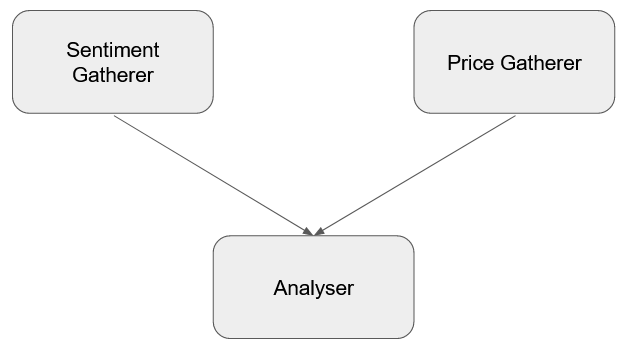
\includegraphics[width=15cm,height=5cm,keepaspectratio]{design/OverallStructure.png}
    \caption{Overall Structure}
    \label{fig:overallstructure}
\end{figure}

\subsection{The Price Gatherer}

The Price Gatherer's purpose is to build a timeline of prices for a given company. It takes in data-points in reference to a given company's prices ordered by date and filters them in order to adapt them to the system. It can be broken down into 3 stages, arranged as seen in figure \ref{fig:pricegathererstructure}:
\begin{itemize}
    \item \texttt{The Price Source} -- Handles the gathering of price values
    \item \texttt{Key Filtering} -- Filters the raw data and extracts the desired keys for each data-point
    \item \texttt{The Return Adder} -- Adds returns to the data-points as extra keys
\end{itemize}

The overall output of this section is an array of JSON objects, ordered by the date key. Each of these objects containing the keys, the exception being the return keys as will be discussed:
\begin{itemize}
    \item \texttt{date} -- the date of the data-point
    \item \texttt{close} -- the closing price for the date of the data-point
    \item \texttt{symbol} -- the symbol representing the company this data is about
    \item \texttt{volume} -- the volume of trades for the date of the data-point
    \item \texttt{return1Day} -- the return in relation to 1 data-point previous
    \item \texttt{return7Day} -- the return in relation to 7 data-points previous
    \item \texttt{return14Day} -- the return in relation to 14 data-points previous
    \item \texttt{return21Day} -- the return in relation to 21 data-points previous
\end{itemize}

\begin{figure}[h]
    \centering
    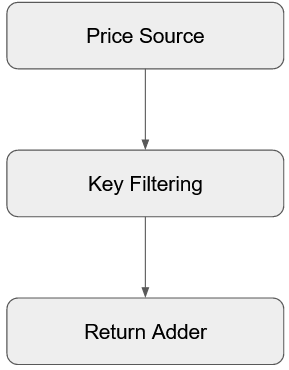
\includegraphics[width=15cm,height=5cm,keepaspectratio]{design/PriceGathererStructure.png}
    \caption{Price Gatherer Structure}
    \label{fig:pricegathererstructure}
\end{figure}

\paragraph{The Price Source}

The purpose of the price source component is to contact the IEX Cloud API and collect daily price points for a given period. Due to the limitations of the tier chosen with the platform, the maximum period allowed is the past 5 years.

\paragraph{Key Filtering}

The IEX Cloud API returns an array of JSON objects, ordered by date, with each object containing the date, close, symbol and volume keys, as well as many others. This component filters out only the desired keys, removing the ones that are not required within the system. This allows the data to managed more easily, as well as any processes being executed faster, and anything that is stored requires less memory. This thus simplifies the process. However, it does create room for future expansion and potential improvement in understanding, as more specificity would be added.

\paragraph{The Return Adder}

The keys missing after the key filtering are those that determine the return values. This component adds them to each entry. The return for a given n determines the difference in closing prices between the current entry and the entry n days before. The returns require previous entries, therefore the first n entries will not have a return given n, the number of previous entries required. The reasoning for adding returns is due to the fact that it allows to examine the change between days rather than the full days themselves, since this project is studying the change in market values.

\subsection{The Sentiment Gatherer}

The Sentiment Gatherer's purpose is to build a timeline of sentiment for a given company. It takes in articles and a dictionary and processes them together in order to create an array of sentiment values ordered by date. It can be broken down into 6 stages, arranged as seen in figure \ref{fig:sentimentgathererstructure}:
\begin{itemize}
    \item \texttt{The Article Source} -- Handles the gathering of articles
    \item \texttt{The Article Parser} -- Parses the raw articles into a format usable by the system
    \item \texttt{The Dictionary} -- Handles the extraction of the dictionary from it's source
    \item \texttt{Key Filtering} -- Filters the dictionary entries and extracts only the desired keys
    \item \texttt{The Sentiment Extractor} -- Uses the dictionary entries in order to extract frequencies of sentiment from the articles
    \item \texttt{Z-Scores} -- Modifies the sentiment extracted from absolute values to relative values using z-scores
\end{itemize}

The overall output of this section is an array of JSON objects, ordered by the date key. Each of these objects containing the keys:
\begin{itemize}
    \item \texttt{date} -- date of the data-point
    \item \texttt{articles} -- z-score of number of articles
    \item \texttt{totalWords} -- z-score of number of total words
    \item \texttt{positiveSentiment} -- z-score of number of positive sentiment words
    \item \texttt{negativeSentiment} -- z-score of number of negative sentiment words
\end{itemize}
The reasoning for using z-scores is due to the fact that it allows to examine the change between days rather than the full days themselves, since this project is studying the change in market values.

TODO - insert diagram

\begin{figure}[h]
    \centering
    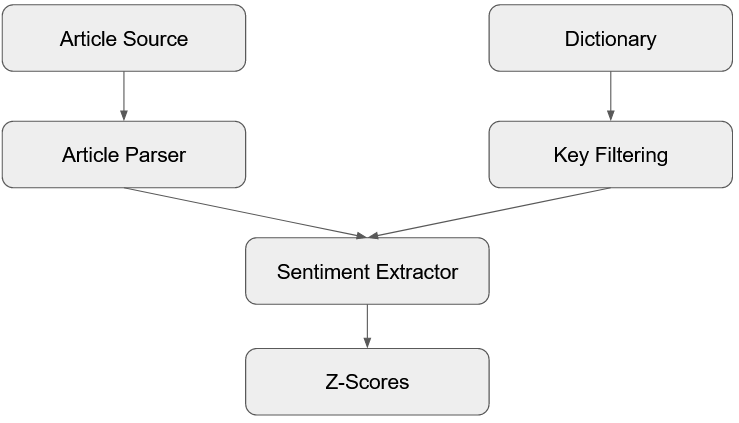
\includegraphics[width=15cm,height=5cm,keepaspectratio]{design/SentimentGathererStructure.png}
    \caption{Sentiment Gatherer Structure}
    \label{fig:sentimentgathererstructure}
\end{figure}

\paragraph{The Article Source}

The purpose of the article source is to provide the articles that will be used in the system.

\paragraph{The Article Parser}

The purpose of this component is to import the files and parse them into a format usable by the system, this being JSON. This is required for LexisNexis as the articles downloaded have the rich text format. The output of this component returns an array of JSON objects, this allows metadata to be stored alongside the body of the article itself.

\paragraph{The Dictionary}

The purpose of this component is to handle the extraction of the dictionary into a JSON object array from the excel sheet it is stored in.

\paragraph{Key Filtering}

The purpose of this component is to filter only the desired keys from the dictionary, in order to decrease processing times and memory requirements. This quite importantly simplifies the analysis significantly. However, it does create room for future expansion and potential improvement in understanding, as more specificity would be added.

\paragraph{The Sentiment Extractor}

The purpose of the component is to extract sentiment frequencies from the articles, using the dictionary as a reference. What this means is that it tallies the number of words belonging to each desired attribute for each article. The articles are then joined by date, tallied appropriately, and ordered by date. The output is an array of JSON objects which represent the absolute values of the different attributes required.

\paragraph{Z-Scores}

The purpose of the component is to take the JSON object produced from the previous component and get the z-scores of the number of articles, of the total number of words in relation to the number of articles, and of each of the sentiment attributes in relation to the total number of words.

\subsection{The Analyser}

There are three components that are predecessors of the main analyser components. These are:
\begin{itemize}
    \item \texttt{The User Interface} -- A command line menu was created in order to organise and utilise all of the various components in a fast and easy way
    \item \texttt{The Joiner} -- It joins the sentiment and prices data-sets where they overlap. Creating two new data-sets.
    \item \texttt{The Period Selector} -- This allows for different periods to be explored within the dataset
\end{itemize}

The Analyser's purpose is to take the timelines produced by the Price Gatherer and the Sentiment Gatherer and analyse them in various different ways. It is a set of unrelated components which allow for the full analysis required in order to understand the data in the way desired for this project. The sub-components build for this component are the following:
\begin{itemize}
    \item \texttt{Return Vs Sentiment Grapher} -- Allows the graphing of sentiment keys and price keys in a time-series
    \item \texttt{Single Point Estimator} -- Uses machine learning model to estimate next day returns
    \item \texttt{Autocorrelator} -- Calculates correlation of key with itself with given lag
    \item \texttt{Return Vs Sentiment Correlator} -- Calculates correlation of given keys with predefined lags
    \item \texttt{Descriptive Statistics} -- Calculates and displays descriptive statistics of given key
    \item \texttt{Vector Autoregressor} -- Calculate Vector Autoregression elements
\end{itemize}

\paragraph{The User Interface}

This is an essential part for the usability of the system create. It allows a user to navigate through the system, and analyse the data in any desired way, given the constraints of the system. It is a set of menu's which allow the selection of any given component and the selected that is desired in the analysis.

\paragraph{The Joiner}

For certain parts of the analysis the data being analysed should be overlapping appropriately. This is an important feature as the price and sentiment data-set have different start and end dates. As well as this not all dates that are covered by one are covered by the other, therefore data must be inserted in these cases, with the assumption that there was no activity for the data that did not exist previously. This has two main cases the first being a day with not sentiment, the assumption can be made that the day has zero sentiment, allowing an appropriate object to be inserted. As for days with no price the assumption can be made that the prices did not vary and the return was 0. However, this case is rare, and no examples of such a situation have been seen.

\paragraph{The Period Selector}

The purpose of this component is quite straight forward. It allows for the narrowing of scope. This is done by allowing for the selection of subsets of the main datasets by selecting a shorted period to examine.

\paragraph{Return Vs Sentiment Grapher}

The purpose of this component is to allow the creation of graphs which compare various columns between the prices data-set and the sentiment data-set. It however also allows the graphing of multiple columns in the one data-set, as well as graphing columns from only one data-set. This allows the creation of any graph desired. The graphs are graphed against the date of the data-point.

\paragraph{Single Point Estimator}

The purpose of this component is to explore the applications of machine learning models in this area. The models take in data from a given date, this being sentiment and price data and estimate whether the nest day would have a positive or negative return. This allows for the comparison between machine learning methods and mathematical methods. The output of this component is two fold. The first item returned is the accuracy of the most accurate model. The second item returned is said model, thus allowing for potential future use and/or storage. This area could be explored in a lot more depth through the use of a more substantial amount of models, hyperparameters and the like.

\paragraph{Autocorrelator}

The autocorrelator allows for the calculation of the correlation of a given column in a given data-set with itself, and it displays the information with n days of lag, where n is selected by the user. This is to help understand how closely related the data is with itself in nearby days, allowing for insight into whether there is a possibility of this data affecting itself. It is important to note, however, that high values of correlation only indicate that there is a potential relationship between days, and does not indicate necessarily causation.

\paragraph{Return Vs Sentiment Correlator}

The return vs sentiment correlator allows for the calculation of three kind of correlation. These are correlation between negative sentiment and 1 day return on the same day, the correlation between these when 1 day return is one day after the negative sentiment, and the correlation between these when negative sentiment is one day after the 1 day return. An expansion to this component would be to allow for different amount of lag between these data-sets. Similarly to the autocorrelator it is important to note, however, that high values of correlation only indicate that there is a potential relationship between elements, and does not indicate necessarily causation.

\paragraph{Descriptive Statistics}

The purpose of the component is to gather a column from the data-set and explore it's descriptive statistics, in order to understand said column better. On top of the descriptive statistics, this component prints out a graph which allows for a visual element. This can be of great aid when trying to understand the significance of the descriptive statistics.

\paragraph{Vector Autoregressor}

The purpose of this component is to explore causation between return and negative sentiment column using vector auto-regression. This adds a layer of rigorousness to the previously explored correlations, as it allows for the understanding of not just what is correlated but which columns cause data in other columns to change. This removes elements such as coincidence.

\section{Scope of Project}

The scope of the project was mainly limited by the data being explored. Many columns were removed from the various data-sources in order to simplify this. The data-set being explored is therefore limited it a general analysis. This can be seen through the use of the generic sentiment columns as well as the basic price columns. On top of this only a certain amount of depth was explored with the machine learning models, correlation and causation. For these reasons I believe there is very large amount of potential expansion to the project, and therefore the understand of the data and its relationships.

\section{Design Summary}

This chapter provides a brief overview of the project, the system design, the handling of the required data and its sources, user interaction with the system, it's design architecture, an explanation of the system components and the scope of the project.
% !TEX root = ../main.tex

\chapter{Implementation}

This chapter outlines and covers the process of implementation of the project. This includes the technologies used for the project, as well as the breakdown of the structure and implementation of the different parts of the project.

\section{Technology Used}

There are various technologies used within this project. These are Python 3.9, Visual Studio Code, Git and Github, Command-Line Interface, AntConc 3.5.9, Rocksteady 0.4 and Gretl. Each of these had a different function within the project.

\subsection{Python 3.9}

Python is an interpreted, high-level and general-purpose programming language. The version used was version 3.9. 

Python was used in this project to develop and execute the procedures outlined in the implementation. This is due to the fact that python is a very useful language for handling projects which require a large amount of various different features as it is general purpose. For that reasons it has many publicly available libraries which help for many of the scenarios come across throughout development.

The libraries used had three main purposes: file handling, data tidying and mathematical operations.

\subsubsection{File Handling}

In order to handle the files downloaded from \emph{lexisnexis} and \emph{proquest}, various libraries and modules had to be used. The libraries and modules being \verb|sys|, \verb|os| and \verb|striprtf|.

The \verb|sys| module provides functions and variables used to manipulate different parts of the Python runtime environment. It is used to create a global variable which allowed the setting of a source for files, and allowed this to be used throughout the various files in the program. The source being the choice between using \emph{lexisnexis} and \emph{proquest} files.

The \verb|os| module provides functions and variables used to perform operating system tasks. It is used to access environment variables, as well as to help parse through files in a given directory.

The \verb|striprtf| library is used to translate rtf to a python string. When files are downloaded from \emph{lexinexis} they are in rtf format. This library is used to help parsed the information in these files into a usable format.

\subsubsection{Data Tidying}

In order to tidy up the data extracted from articles and make it usable in the context required the use of some libraries is needed. These libraries and modules are \verb|pandas|, \verb|json|, \verb|copy|, \verb|datetime|, \verb|operator|, \verb|matplotlib|, \verb|seaborn| and \verb|warnings|.

The \verb|pandas| is an open source data analysis and manipulation tool. This library is used to aid in the tabling of data. This was useful in order to use this data within graphs and to create an excel spreadsheet. For graphing timeseries, this library was especially useful with it's \verb|to_datetime()| function which allowed the dates to be appropriately used as indices. This is significant especially when comparing two separate time series, as it spaced the values according to date and not which datapoint it is along the sequence.

The \verb|json| library is used to dump json data from files and the extract it back from the file in order to cache the information extracted for future use.

The \verb|copy| library is used to create deepcopies of json objects. This is necessary as the copies had to be completely separate from the original version, and due to how python works this cannot simply be done through a shallow copy. Therefore the library was used to facilitate this.

The \verb|datetime| module supplies classes for manipulating dates and times. As they are usually stored in strings they can be complex to perform operations with. The library makes this process a lot more straightforward.

The \verb|operator| module exports a set of efficient functions corresponding to the intrinsic operators of Python. It is used sort arrays of json objects that contain a given key. This was very useful when ordering data entries by date.

The \verb|matplotlib| library provides an object-oriented API for embedding plots into applications using general-purpose GUI toolkits like Tkinter, wxPython, Qt, or GTK. It therefore aids in the creation and display of graphs within the system.

The \verb|seaborn| library is a data visualization library based on matplotlib. It helps the graphs look more aesthetically pleasing as well helping them become cleaere, therefore easier to read.

The \verb|warnings| module is used in order to supress warnings. This helps make the program be easier to read for an end user.

\subsubsection{Mathematical Operations}

In order to perform mathematical operations appropriately multiple libraries are used. This is to avoid the recreation of tested and efficient functions, and avoid any potential errors when recreating them. These libraries and modules are \verb|numpy|, \verb|statistics|, \verb|scipy|, \verb|math|, \verb|sklearn| and \verb|time|.

The \verb|numpy| is a Python library used for working with arrays. It also has functions for working in domain of linear algebra, fourier transform, and matrices.

The \verb|statistics| is a built-in Python library for descriptive statistics.

The \verb|scipy| is a collection of mathematical algorithms and convenience functions built on the \verb|numpy| extension of Python. It adds significant power to the interactive Python session by providing the user with high-level commands and classes for manipulating and visualizing data. Specifically the \verb|scipy.stats| module was used. Similarly, to the \verb|statistics| library it was used to gather various types of statistical information.

The \verb|math| module is a built-in module that you can use for mathematical tasks. It is used specifically for the \verb|log()| function contained within.

The \verb|sklearn| library is an incredibly useful machine learning library. The \verb|sklearn| library contains a lot of efficient tools for machine learning and statistical modeling including classification, regression, clustering and dimensionality reduction. It is used for the machine learning functionality required for the \verb|singlePointEstimator|. These being various trainable models, appropriately metric measuring functions, and some utility functions.

The \verb|time| module provides various time-related functions. Most of the functions defined in this module call platform C library functions with the same name. This important because it is used to time some elements of the system, and these timings must be precise.

\subsection{Visual Studio Code}

Visual Studio Code is a freeware source-code editor made by Microsoft for Windows, Linux and macOS. Features include support for debugging, syntax highlighting, intelligent code completion, snippets, code refactoring, and embedded Git. It was used to ease the development of the codebase.

\subsection{Git and Github}

Git is a version control system. Git tracks the changes you make to files, so you have a record of what has been done, and you can revert to specific versions should you ever need to. Git allows changes by multiple people to all be merged into one source. This can be used to create features then once they are complete merge them into a final version of the system.

GitHub is a provider of Internet hosting for software development and version control using Git. It offers the distributed version control and source code management functionality of Git, plus its own features.

\subsection{Command-Line Interface}

A command-line interface processes commands to a computer program in the form of lines of text. It is used to execute the programs developed, git commands and any other required commands.

\subsection{AntConc 3.5.9}

AntConc is a freeware corpus analysis toolkit for concordancing and text analysis. It is used for preliminary text analysis of the articles downloaded from \emph{lexisnexis} and \emph{proquest}. It can be used to create words lists, n-grams, concordance plots, amongst other useful tools that may be used to examine word choices in texts.

\subsection{Rocksteady 0.4}

Rocksteady is a sentiment analysis tool. It creates a timeline of sentiment, and allows the filtering as well as visualisation of this data. It is used within this project to understand how the sentiment proxy extraction process works.

\subsection{Gretl}

Gretl is an open-source statistical package, mainly for econometrics. The name is an acronym for Gnu Regression, Econometrics and Time-series Library. It has both a graphical user interface and a command-line interface. It was mainly used for vector autoregression within this project.

\section{Setting up the System}

The technologies that have been used to implement the system have been covered. This section therefore covers the details of the implementation of the indivdual components laid out in the design, using these technologies.

The system is run as a script using the terminal. The commmand for initiating the program being \verb|python IntelligentAnalysis.py|. This is assuming that the default version of python running is version 3.9, otherwise the command may have to be modified slightly to accomodate for this. The full codebase can be found at the following url: \url{https://github.com/DaVinciTachyon/FinalYearProject}. This command is run from the root directory of this git repository.

\subsection{The Price Gatherer}
TODO what? why? how?
\subsubsection{The Price Source}
TODO what? why? how?
\subsubsection{Key Filtering}
TODO what? why? how?
\subsubsection{The Return Adder}
TODO what? why? how?
\subsection{The Sentiment Gatherer}
TODO what? why? how?
\subsubsection{The Article Source}
TODO what? why? how?
\subsubsection{The Article Parser}
TODO what? why? how?
\subsubsection{The Dictionary}
TODO what? why? how?
\subsubsection{Key Filtering}
TODO what? why? how?
\subsubsection{The Sentiment Extractor}
TODO what? why? how?
\subsubsection{Z-Scores}
TODO what? why? how?
\subsection{The Analyser}
TODO what? why? how?
\subsubsection{The User Interface}
TODO what? why? how?
\subsubsection{The Joiner}
TODO what? why? how?
\subsubsection{Return Vs Sentiment Grapher}
TODO what? why? how?
\subsubsection{Single Point Estimator}
TODO what? why? how?
\subsubsection{Autocorrelator}
TODO what? why? how?
\subsubsection{Return Vs Sentiment Correlator}
TODO what? why? how?
\subsubsection{Descriptive Statistics}
TODO what? why? how?
\subsubsection{Vector Autoregressor}
TODO what? why? how?
\section{Implementation Summary}
TODO what? why? how?
% !TEX root = ../main.tex

\chapter{Results Evaluation}
TODO what? why? how?
\section{}
TODO what? why? how?
\section{Results Evaluation Summary}
TODO what? why? how?
% !TEX root = ../main.tex

\chapter{Discussion \& Conclusion}

In this chapter, the questions explored and the way they are answered is explored, the success to which they have been answered, and how the challenges put in the way were overcome. There will also be an outline of potential continued work in the area.

\section{Project Achievements}

TODO what? why? how?
it should examine what has been achieved in the project and relate this to the initial aim of the project
Do not be afraid to discuss disadvantages of your approach. Negative results are useful

restate questions
achievements
what I have learnt
advantages of approach
disadvantages of approach

\section{Challenges}

TODO what? why? how?
Any problems encountered in the course of the project should be mentioned here

\section{Future Work}

TODO what? why? how?
The section on future work should give some indication of how work done could be improved and developed

\section{Discussion \& Conclusion Summary}

TODO what? why? how?
\bibliographystyle{unsrtnat}
\bibliography{bibs/sample}
\appendix
\renewcommand{\thechapter}{A\arabic{chapter}}
% !TEX root = ../main.tex

\chapter{Appendix}

The appendix contains extensions upon the information in the rest of the text. However, this information was not necessary to reach the desired conclusions in the text.

\section{Descriptive Statistics}
\label{appendix:descriptiveStatistics}

\subsection{Closing Prices}

\subsubsection{Entire Dataset}

\begin{figure}[h!]
    \centering
    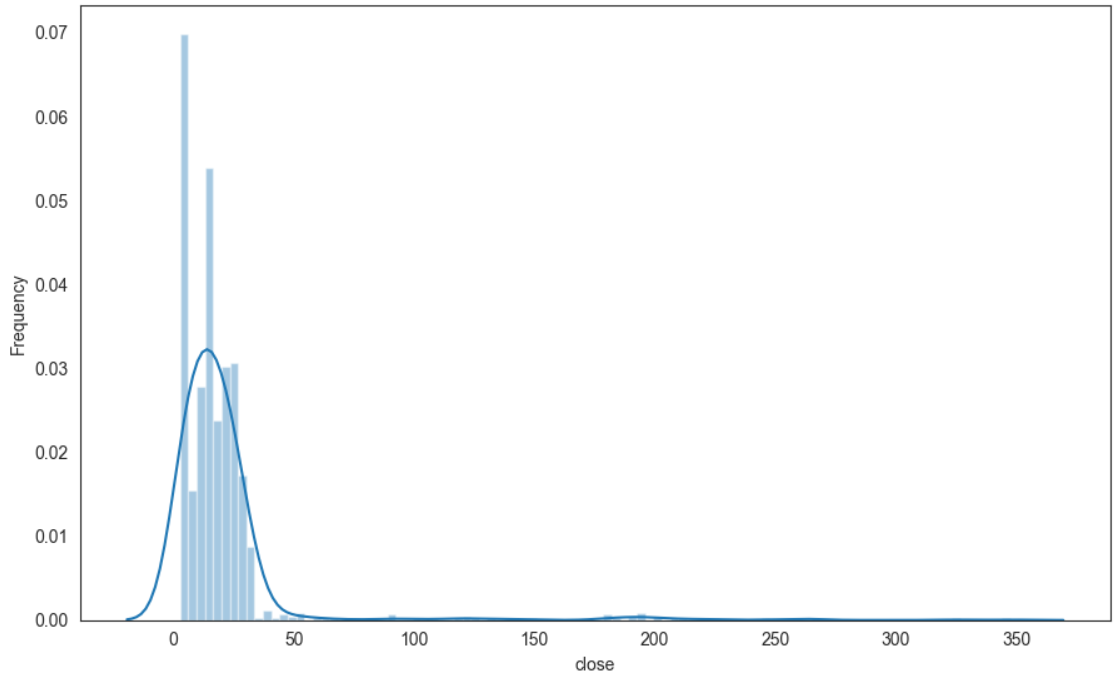
\includegraphics[width=15cm,height=7cm,keepaspectratio]{resultsEvaluation/closeDescMax.png}
    \caption{Closing Prices with entire dataset}
    \label{fig:appendix_closeDescMax}
\end{figure}
\begin{center}
\begin{tabular}{ c c }
\hline
\multicolumn{2}{|c|}{Closing Price Descriptive Statistics with entire dataset} \\
\hline
Mean & 20.25539316918189 \\
Standard Error & 0.8617871146224114 \\
Median & 15.22 \\
Mode & 4.14 \\
Standard Deviation & 30.56612021354625 \\
Sample Variance & 935.0303819398896 \\
Kurtosis & 43.00117239290764 \\
Skewness & 6.080884821536175 \\
Range & 344.71 \\
Minimum & 2.8 \\
Maximum & 347.51 \\
Sum & 25501.540000000005 \\
Count & 1259  
\end{tabular}
\end{center}

\subsubsection{Last Year}

\begin{figure}[h!]
    \centering
    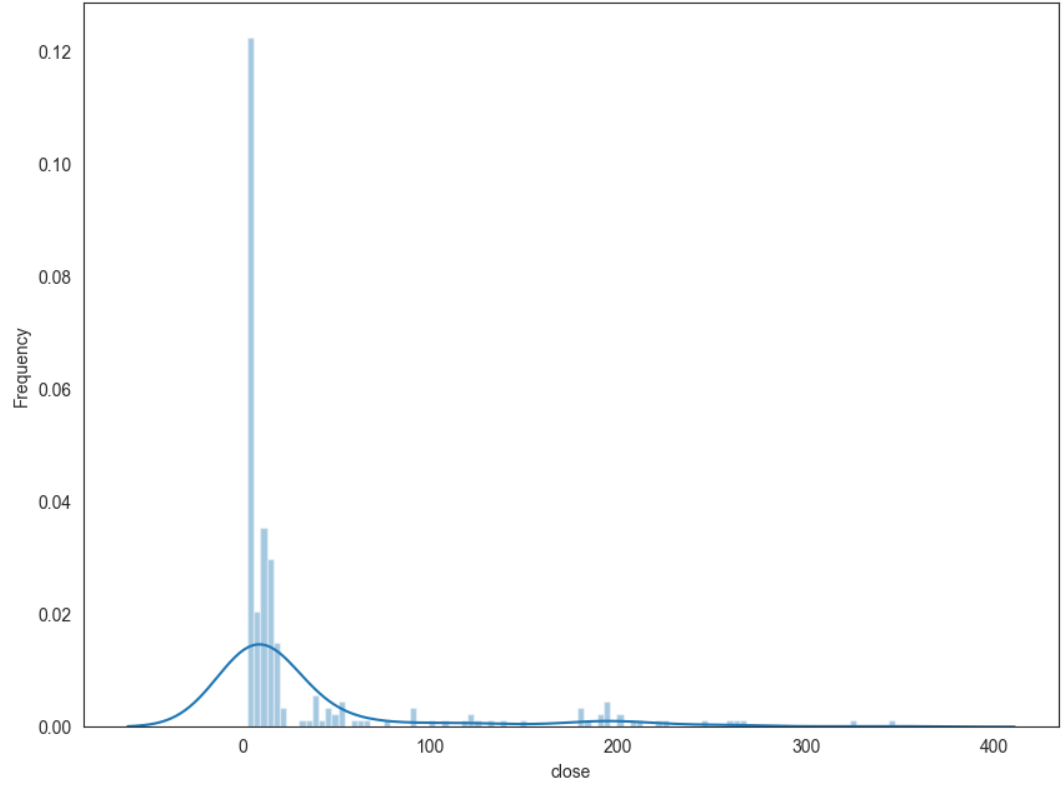
\includegraphics[width=15cm,height=7cm,keepaspectratio]{resultsEvaluation/closeDesc1.png}
    \caption{Closing Prices in the last year of data}
    \label{fig:appendix_closeDesc1}
\end{figure}
\begin{center}
\begin{tabular}{ c c }
\hline
\multicolumn{2}{|c|}{Closing Price Descriptive Statistics in the last year of data} \\
\hline
Mean & 35.32043478260869 \\
Standard Error & 4.034091200037088 \\
Median & 10.02 \\
Mode & 4.44 \\
Standard Deviation & 64.03921248871352 \\
Sample Variance & 4117.294627984817 \\
Kurtosis & 6.11122201031286 \\
Skewness & 2.5837008559997834 \\
Range & 344.71 \\
Minimum & 2.8 \\
Maximum & 347.51 \\
Sum & 8936.07 \\
Count & 253
\end{tabular}
\end{center}

\subsection{Trading Volume}

\subsubsection{Entire Dataset}

\begin{figure}[h!]
    \centering
    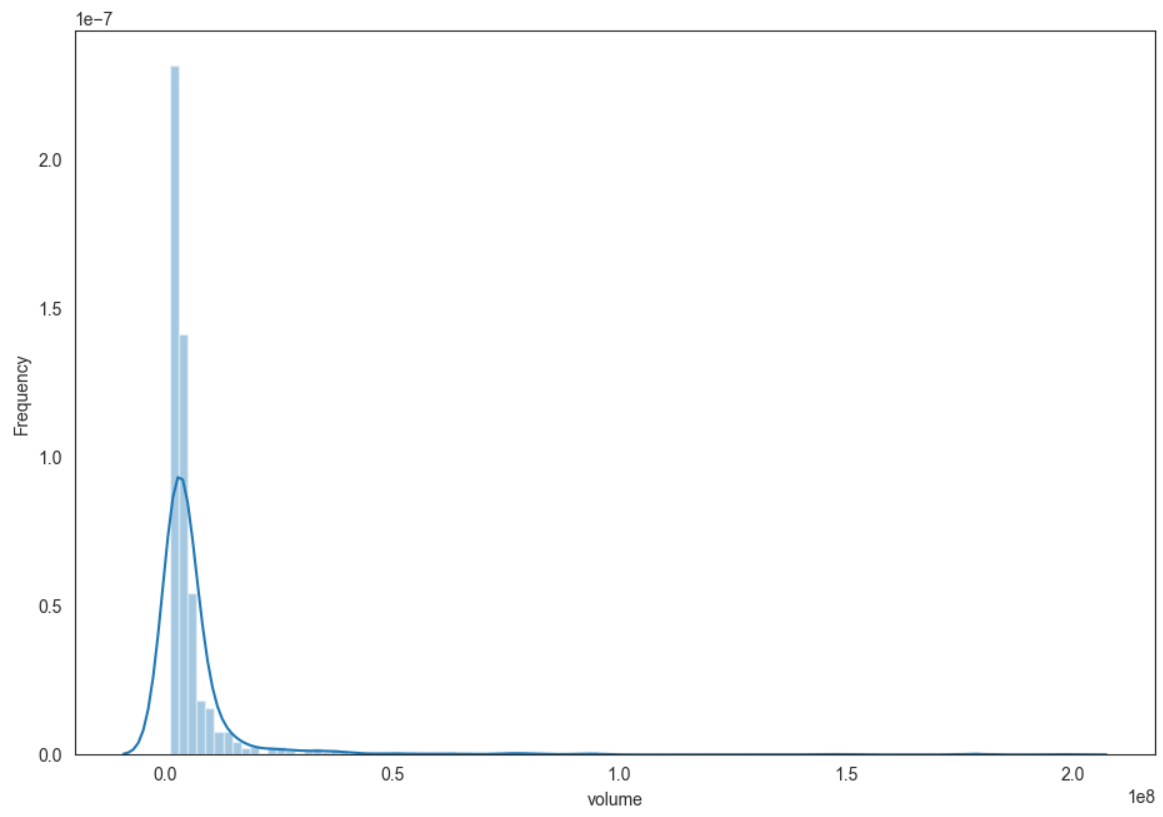
\includegraphics[width=15cm,height=7cm,keepaspectratio]{resultsEvaluation/volumeDescMax.png}
    \caption{Trading Volume with entire dataset}
    \label{fig:appendix_volumeDescMax}
\end{figure}
\begin{center}
\begin{tabular}{ c c }
\hline
\multicolumn{2}{|c|}{Trading Volume Descriptive Statistics with entire dataset} \\
\hline
Mean & 6435867.801429706 \\
Standard Error & 399372.9943423072 \\
Median & 3130713 \\
Mode & 1491760 \\
Standard Deviation & 14165079.458700724 \\
Sample Variance & 200808974859915.2 \\
Kurtosis & 81.30752829995787 \\
Skewness & 8.021781388564962 \\
Range & 196185042 \\
Minimum & 972904 \\
Maximum & 197157946 \\
Sum & 8102757562 \\
Count & 1259
\end{tabular}
\end{center}

\subsubsection{Last Year}

\begin{figure}[h!]
    \centering
    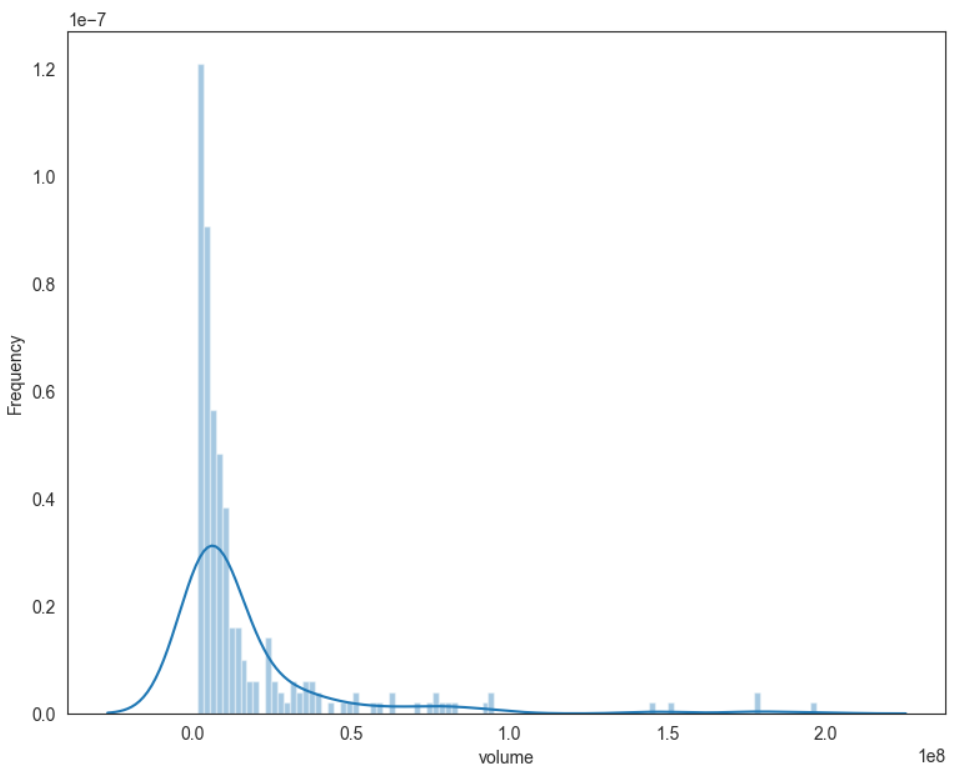
\includegraphics[width=15cm,height=7cm,keepaspectratio]{resultsEvaluation/volumeDesc1.png}
    \caption{Trading Volume in the last year of data}
    \label{fig:appendix_volumeDesc1}
\end{figure}
\begin{center}
\begin{tabular}{ c c }
\hline
\multicolumn{2}{|c|}{Trading Volume Descriptive Statistics in the last year of data} \\
\hline
Mean & 16731690.841897232 \\
Standard Error & 1798626.81876273 \\
Median & 6603951 \\
Mode & 4568695 \\
Standard Deviation & 28552315.58314456 \\
Sample Variance & 818469783592652.2 \\
Kurtosis & 16.215823114980463 \\
Skewness & 3.730320402302758 \\
Range & 195827485 \\
Minimum & 1330461 \\
Maximum & 197157946 \\
Sum & 4233117783 \\
Count & 253
\end{tabular}
\end{center}

\subsection{1 Day Returns}

\subsubsection{Entire Dataset}

\begin{figure}[h!]
    \centering
    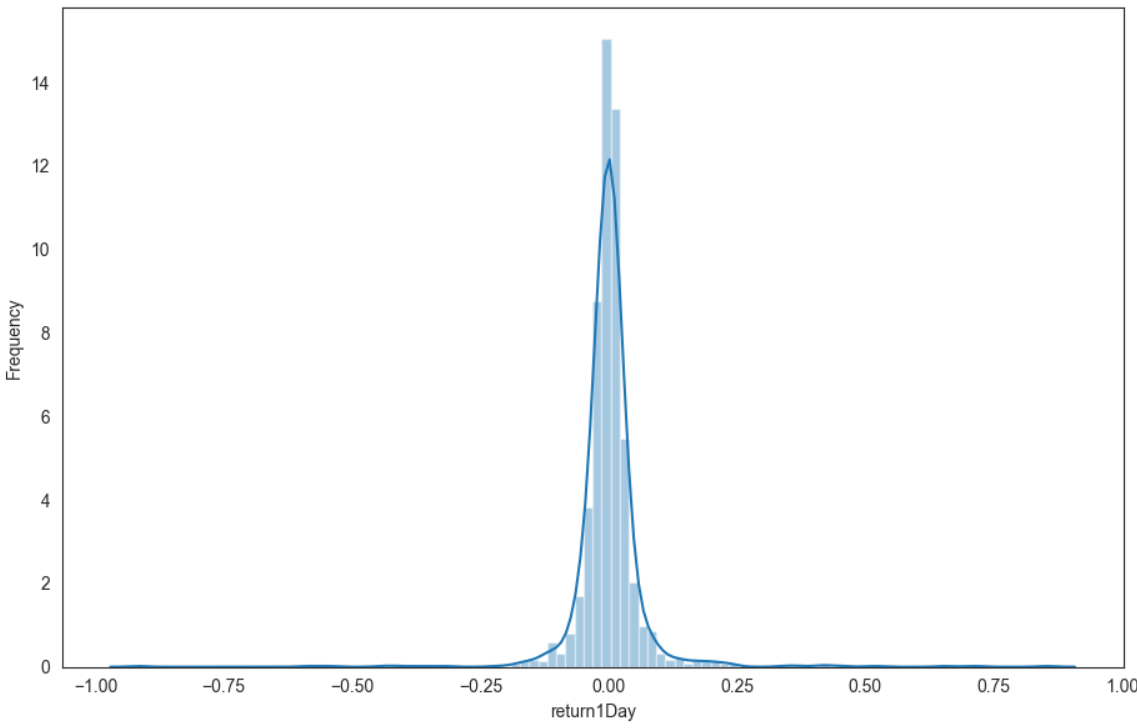
\includegraphics[width=15cm,height=7cm,keepaspectratio]{resultsEvaluation/1returnDescMax.png}
    \caption{1 Day Returns with entire dataset}
    \label{fig:appendix_1returnDescMax}
\end{figure}
\begin{center}
\begin{tabular}{ c c }
\hline
\multicolumn{2}{|c|}{1 Day Return Descriptive Statistics with entire dataset} \\
\hline
Mean & 0.0014490461774454091 \\
Standard Error & 0.0021291609999713954 \\
Median & 0.0 \\
Mode & 0.0 \\
Standard Deviation & 0.07548769098797223 \\
Sample Variance & 0.005702924817259385 \\
Kurtosis & 51.56501043384626 \\
Skewness & 0.7637560467880287 \\
Range & 1.770007043945965 \\
Minimum & -0.916290731874155 \\
Maximum & 0.85371631207181 \\
Sum & 1.8229000912263227 \\
Count & 1258
\end{tabular}
\end{center}

\subsubsection{Last Year}

\begin{figure}[h!]
    \centering
    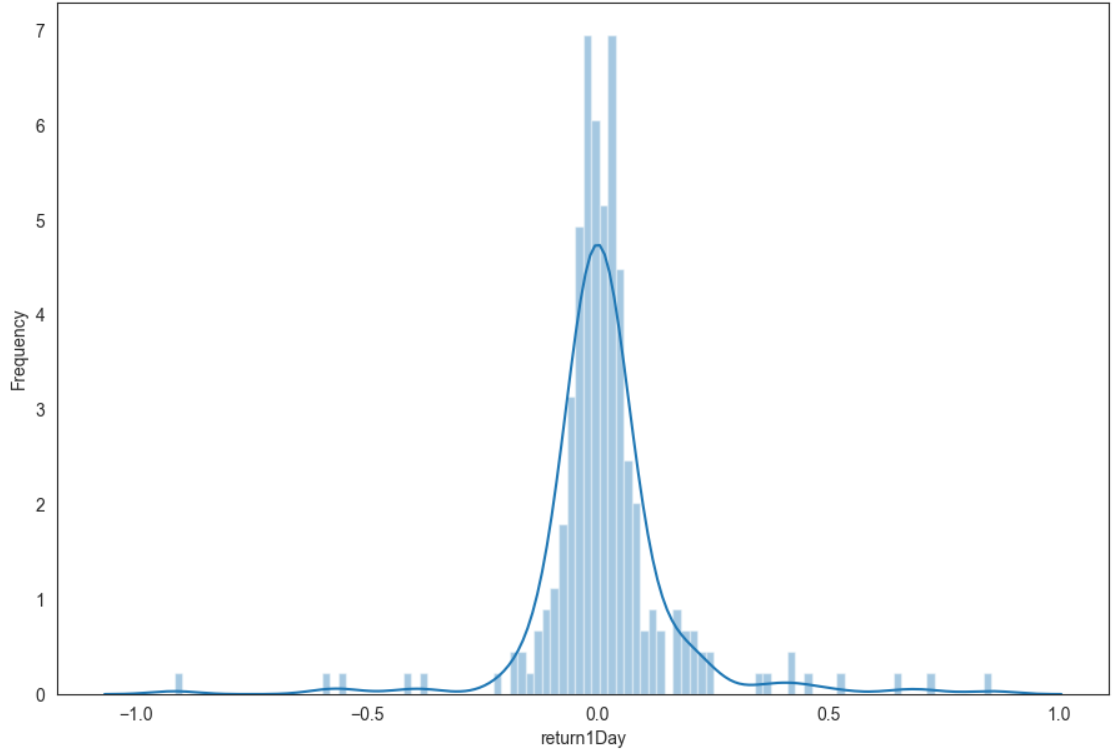
\includegraphics[width=15cm,height=7cm,keepaspectratio]{resultsEvaluation/1returnDesc1.png}
    \caption{1 Day Returns in the last year of data}
    \label{fig:appendix_1returnDesc1}
\end{figure}
\begin{center}
\begin{tabular}{ c c }
\hline
\multicolumn{2}{|c|}{1 Day Return Descriptive Statistics in the last year of data} \\
\hline
Mean & 0.01617449079992721 \\
Standard Error & 0.009609836418644279 \\
Median & 0.005313187705878563 \\
Mode & 0.022335953942063298 \\
Standard Deviation & 0.15224844154955602 \\
Sample Variance & 0.02327193691026168 \\
Kurtosis & 12.867982373920272 \\
Skewness & 0.32394336153811276 \\
Range & 1.770007043945965 \\
Minimum & -0.916290731874155 \\
Maximum & 0.85371631207181 \\
Sum & 4.075971681581655 \\
Count & 252
\end{tabular}
\end{center}

\subsection{Article Volume}

\subsubsection{Entire Dataset}

\begin{figure}[h!]
    \centering
    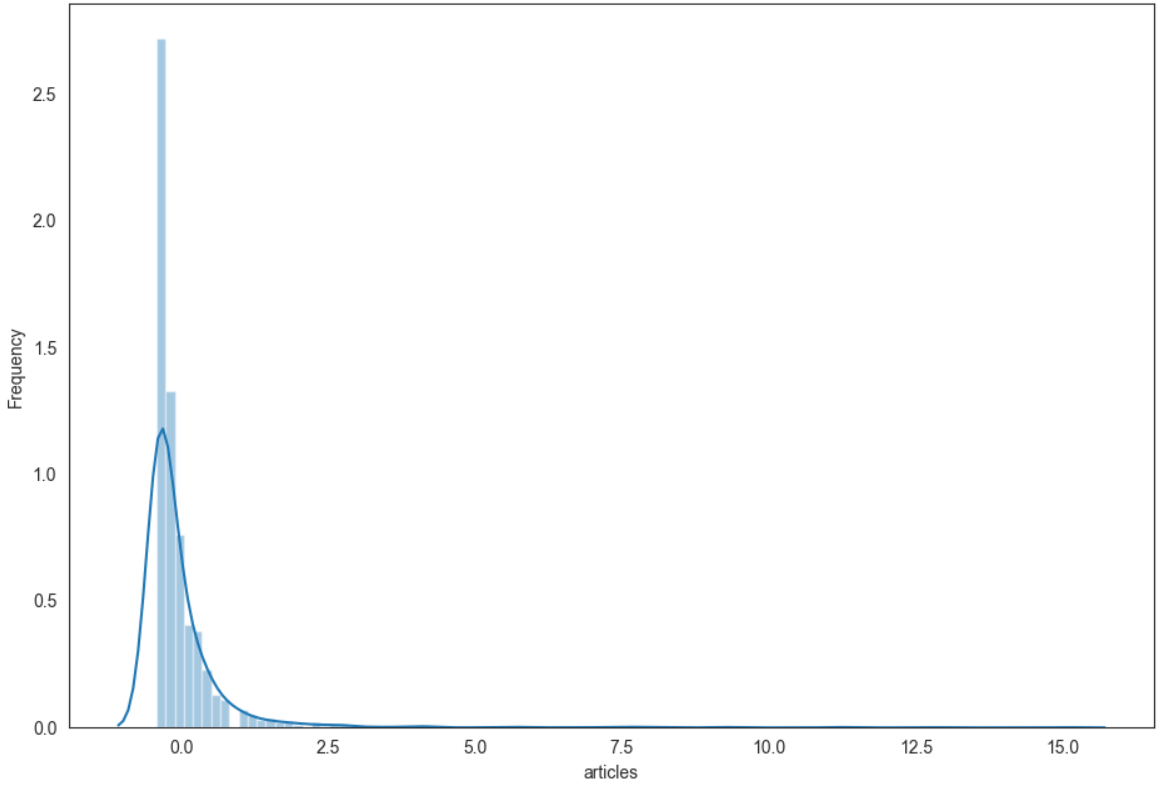
\includegraphics[width=15cm,height=7cm,keepaspectratio]{resultsEvaluation/articleDescMax.png}
    \caption{Article Volume with entire dataset}
    \label{fig:appendix_articleDescMax}
\end{figure}
\begin{center}
\begin{tabular}{ c c }
\hline
\multicolumn{2}{|c|}{Article Volume Descriptive Statistics with entire dataset} \\
\hline
Mean & -2.2065213996409285e-17 \\
Standard Error & 0.02196873875818734 \\
Median & -0.2421631034547878 \\
Mode & -0.41805802758295 \\
Standard Deviation & 1.0 \\
Sample Variance & 1.0004826254826256 \\
Kurtosis & 73.76924857053827 \\
Skewness & 7.360900854018193 \\
Range & 15.478753323278276 \\
Minimum & -0.41805802758295 \\
Maximum & 15.060695295695327 \\
Sum & -4.642022877199281e-12 \\
Count & 2073
\end{tabular}
\end{center}

\subsubsection{Last Year}

\begin{figure}[h!]
    \centering
    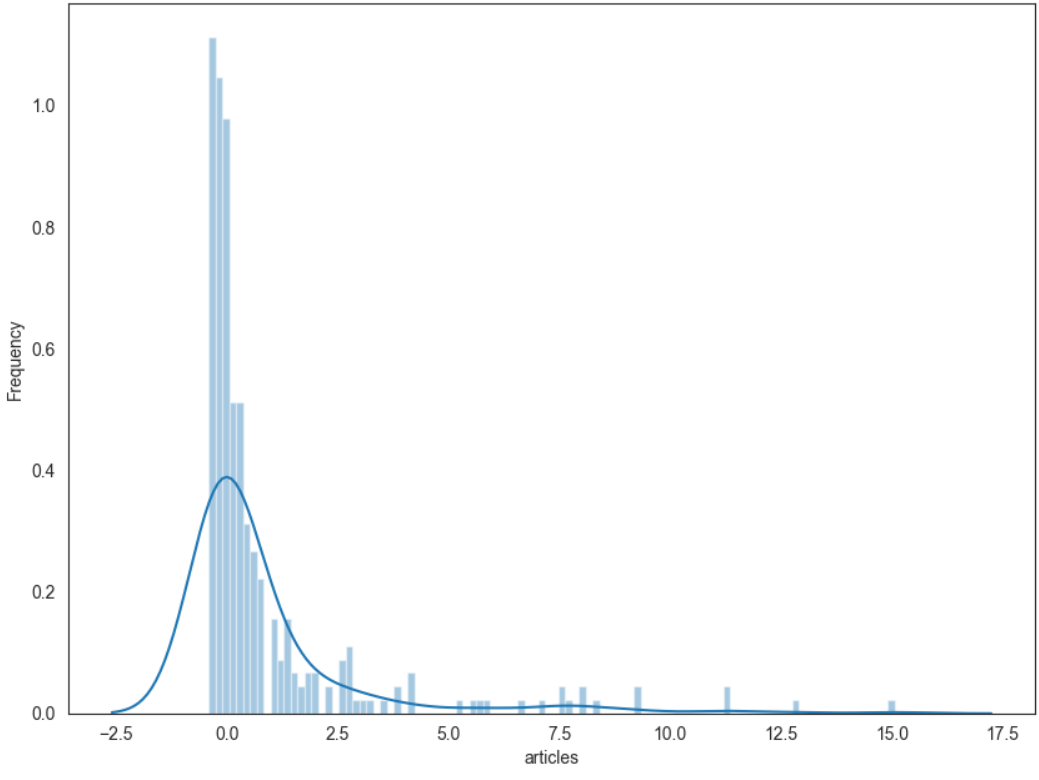
\includegraphics[width=15cm,height=7cm,keepaspectratio]{resultsEvaluation/articleDesc1.png}
    \caption{Article Volume in the last year of data}
    \label{fig:appendix_articleDesc1}
\end{figure}
\begin{center}
\begin{tabular}{ c c }
\hline
\multicolumn{2}{|c|}{Article Volume Descriptive Statistics in the last year of data} \\
\hline
Mean & 0.8623357132258448 \\
Standard Error & 0.1325148497318309 \\
Median & 0.1096267448015367 \\
Mode & -0.41805802758295 \\
Standard Deviation & 2.2527524454411254 \\
Sample Variance & 5.092453765840419 \\
Kurtosis & 12.21615870052046 \\
Skewness & 3.296079615884022 \\
Range & 15.478753323278276 \\
Minimum & -0.41805802758295 \\
Maximum & 15.060695295695327 \\
Sum & 250.07735683549507 \\
Count & 290
\end{tabular}
\end{center}

\subsection{Words Volume}

\subsubsection{Entire Dataset}

\begin{figure}[h!]
    \centering
    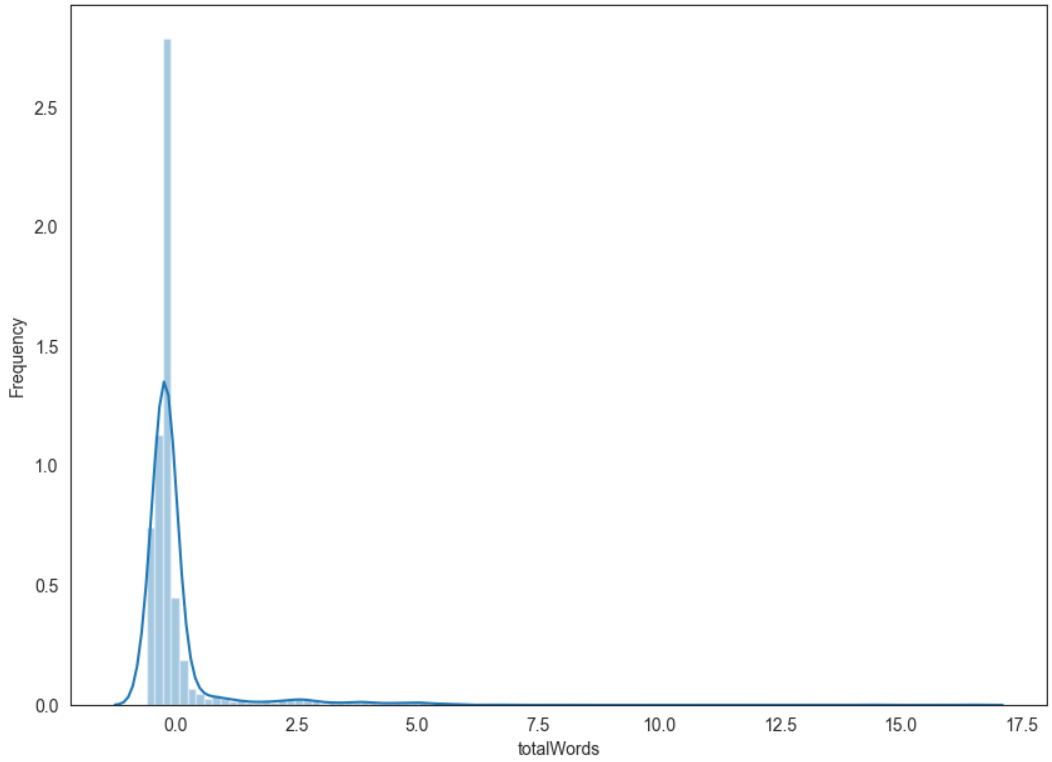
\includegraphics[width=15cm,height=7cm,keepaspectratio]{resultsEvaluation/wordsDescMax.png}
    \caption{Words Volume with entire dataset}
    \label{fig:appendix_wordsDescMax}
\end{figure}
\begin{center}
\begin{tabular}{ c c }
\hline
\multicolumn{2}{|c|}{Words Volume Descriptive Statistics with entire dataset} \\
\hline
Mean & 0.00013989387361311993 \\
Standard Error & 0.021968180574674083 \\
Median & -0.2 \\
Mode & -0.19 \\
Standard Deviation & 0.999974591918116 \\
Sample Variance & 1.0004317854395641 \\
Kurtosis & 66.70204164146547 \\
Skewness & 6.45609886055835 \\
Range & 17.07 \\
Minimum & -0.61 \\
Maximum & 16.46 \\
Sum & 0.28999999999995796 \\
Count & 2073
\end{tabular}
\end{center}

\subsubsection{Last Year}

\begin{figure}[h!]
    \centering
    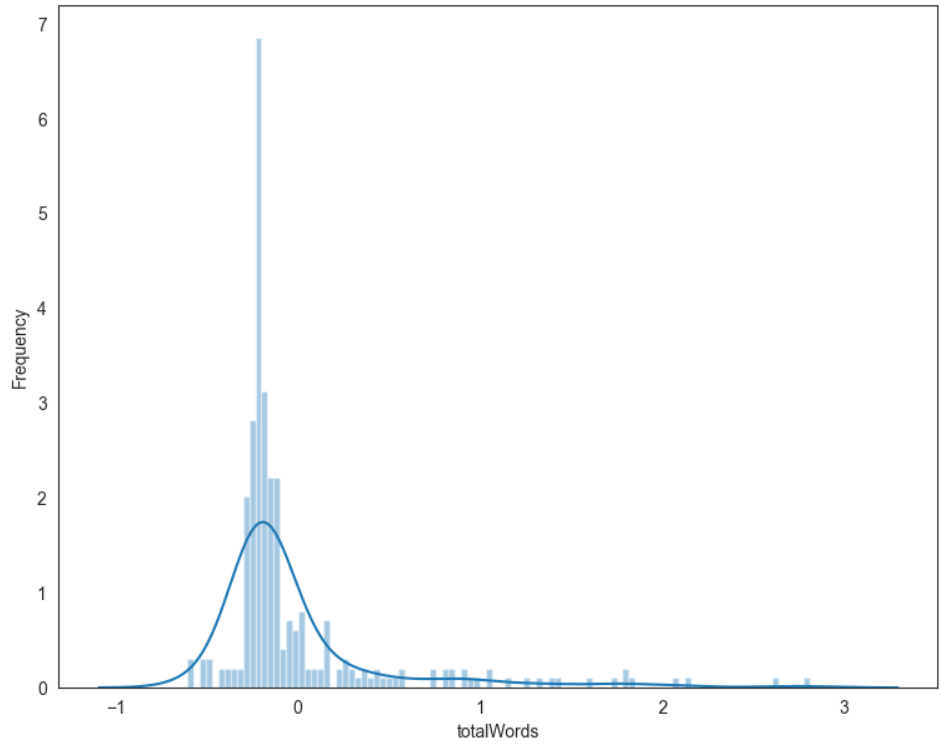
\includegraphics[width=15cm,height=7cm,keepaspectratio]{resultsEvaluation/wordsDesc1.png}
    \caption{Words Volume in the last year of data}
    \label{fig:appendix_wordsDesc1}
\end{figure}
\begin{center}
\begin{tabular}{ c c }
\hline
\multicolumn{2}{|c|}{Words Volume Descriptive Statistics in the last year of data} \\
\hline
Mean & -0.010758620689655175 \\
Standard Error & 0.029379055463608056 \\
Median & -0.19 \\
Mode & -0.22 \\
Standard Deviation & 0.4994439428813369 \\
Sample Variance & 0.2503073809807899 \\
Kurtosis & 9.61184972410166 \\
Skewness & 2.9411586965134755 \\
Range & 3.42 \\
Minimum & -0.61 \\
Maximum & 2.81 \\
Sum & -3.1200000000000068 \\
Count & 290
\end{tabular}
\end{center}

\subsection{Positive Sentiment}

\subsubsection{Entire Dataset}

\begin{figure}[h!]
    \centering
    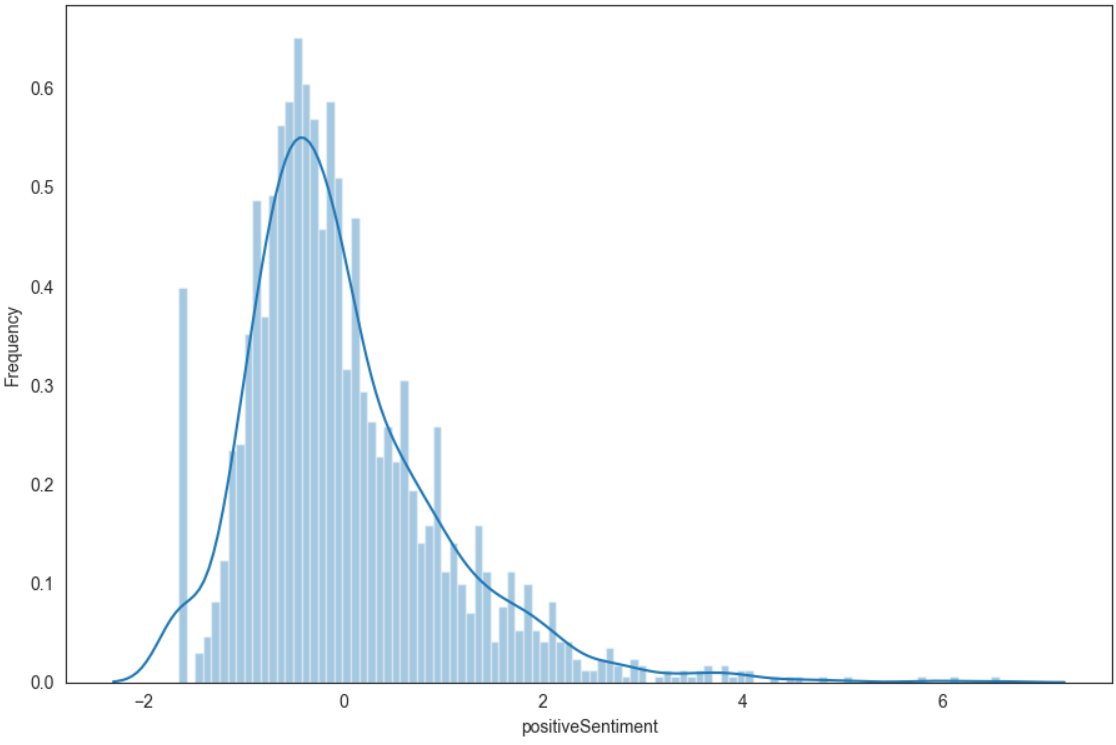
\includegraphics[width=15cm,height=7cm,keepaspectratio]{resultsEvaluation/positiveDescMax.png}
    \caption{Positive Sentiment with entire dataset}
    \label{fig:appendix_positiveDescMax}
\end{figure}
\begin{center}
\begin{tabular}{ c c }
\hline
\multicolumn{2}{|c|}{Positive Sentiment Descriptive Statistics with entire dataset} \\
\hline
Mean & -0.00011577424023154774 \\
Standard Error & 0.021969944580020426 \\
Median & -0.21 \\
Mode & -1.65 \\
Standard Deviation & 1.0000548880773885 \\
Sample Variance & 1.0005924576323273 \\
Kurtosis & 4.061676439612937 \\
Skewness & 1.4873401549309522 \\
Range & 8.22 \\
Minimum & -1.65 \\
Maximum & 6.57 \\
Sum & -0.23999999999965826 \\
Count & 2073
\end{tabular}
\end{center}

\subsubsection{Last Year}

\begin{figure}[h!]
    \centering
    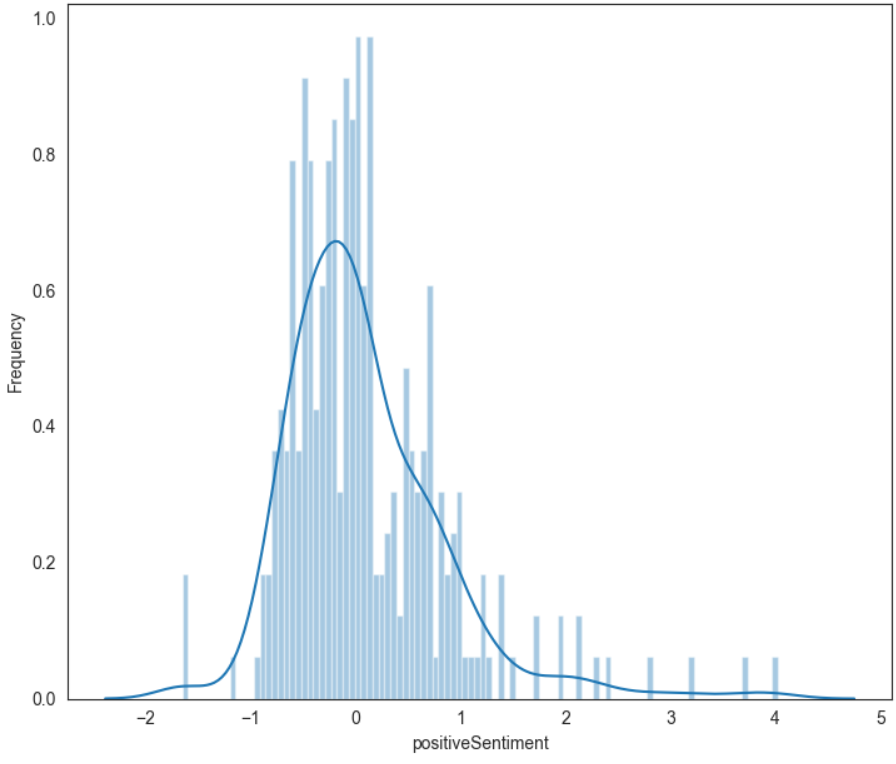
\includegraphics[width=15cm,height=7cm,keepaspectratio]{resultsEvaluation/positiveDesc1.png}
    \caption{Positive Sentiment in the last year of data}
    \label{fig:appendix_positiveDesc1}
\end{figure}
\begin{center}
\begin{tabular}{ c c }
\hline
\multicolumn{2}{|c|}{Positive Sentiment Descriptive Statistics in the last year of data} \\
\hline
Mean & 0.0863103448275862 \\
Standard Error & 0.04453127962901483 \\
Median & -0.055 \\
Mode & -0.1 \\
Standard Deviation & 0.7570317536932523 \\
Sample Variance & 0.5750801109652786 \\
Kurtosis & 5.009115638344465 \\
Skewness & 1.636685164397725 \\
Range & 5.67 \\
Minimum & -1.65 \\
Maximum & 4.02 \\
Sum & 25.029999999999973 \\
Count & 290
\end{tabular}
\end{center}

\subsection{Negative Sentiment}

\subsubsection{Entire Dataset}

\begin{figure}[h!]
    \centering
    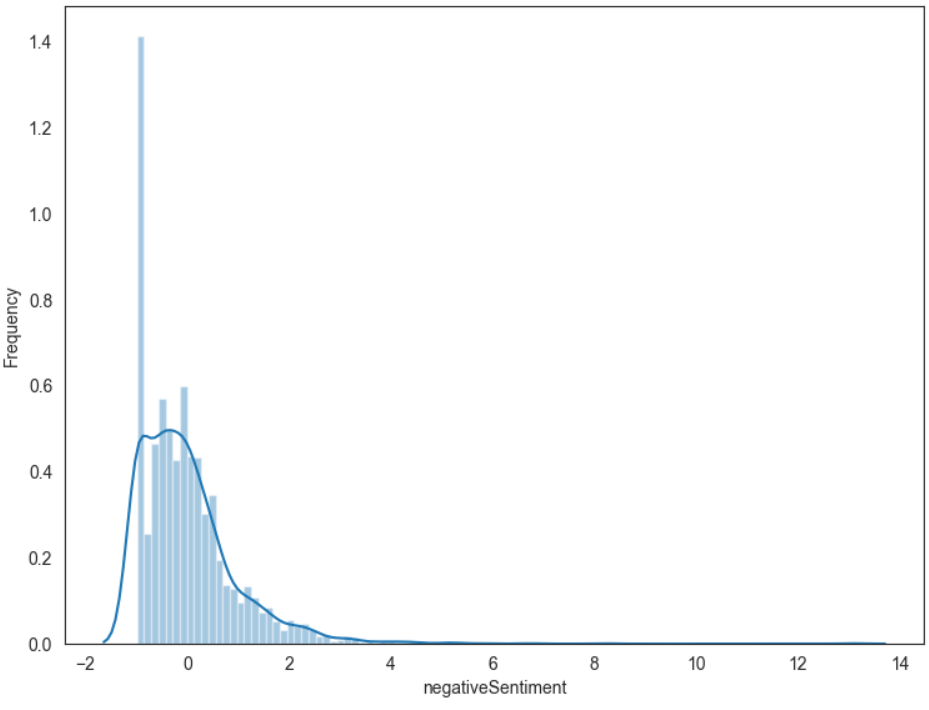
\includegraphics[width=15cm,height=7cm,keepaspectratio]{resultsEvaluation/negativeDescMax.png}
    \caption{Negative Sentiment with entire dataset}
    \label{fig:appendix_negativeDescMax}
\end{figure}
\begin{center}
\begin{tabular}{ c c }
\hline
\multicolumn{2}{|c|}{Negative Sentiment Descriptive Statistics with entire dataset} \\
\hline
Mean & 0.00014471780028943782 \\
Standard Error & 0.021964634770156394 \\
Median & -0.17 \\
Mode & -0.99 \\
Standard Deviation & 0.9998131896384166 \\
Sample Variance & 1.000108859355531 \\
Kurtosis & 19.513842113440127 \\
Skewness & 2.77912574439437 \\
Range & 14.05 \\
Minimum & -0.99 \\
Maximum & 13.06 \\
Sum & 0.30000000000174065 \\
Count & 2073
\end{tabular}
\end{center}

\subsubsection{Last Year}

\begin{figure}[h!]
    \centering
    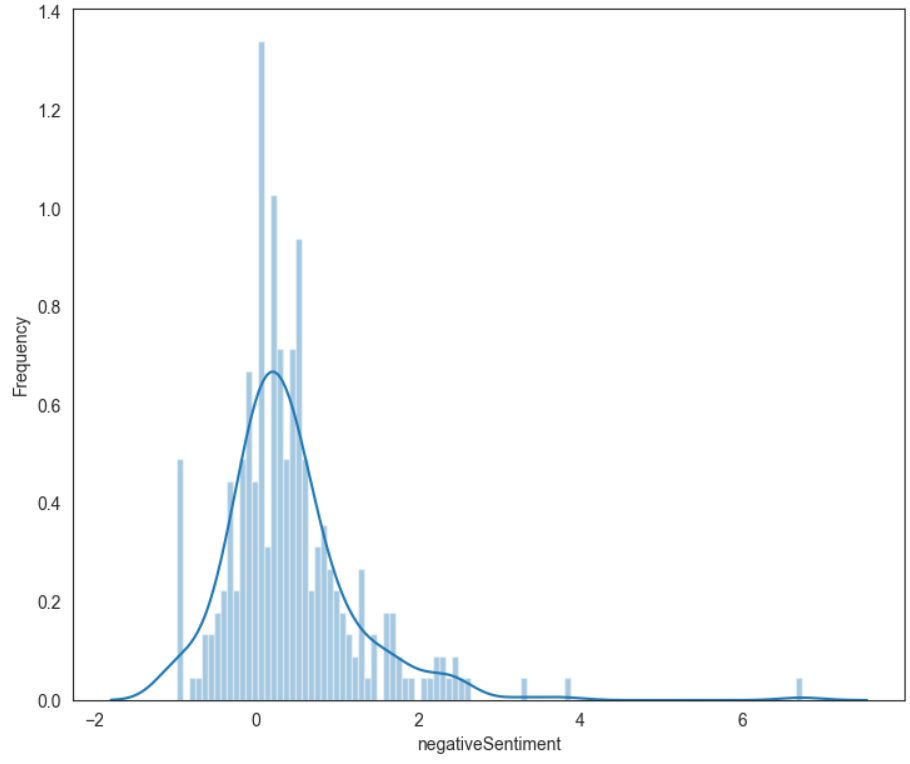
\includegraphics[width=15cm,height=7cm,keepaspectratio]{resultsEvaluation/negativeDesc1.png}
    \caption{Negative Sentiment in the last year of data}
    \label{fig:appendix_negativeDesc1}
\end{figure}
\begin{center}
\begin{tabular}{ c c }
\hline
\multicolumn{2}{|c|}{Negative Sentiment Descriptive Statistics in the last year of data} \\
\hline
Mean & 0.41293103448275864 \\
Standard Error & 0.04888104930864328 \\
Median & 0.27 \\
Mode & 0.08 \\
Standard Deviation & 0.8309778382469358 \\
Sample Variance & 0.6929135246390645 \\
Kurtosis & 11.895721323794636 \\
Skewness & 2.2637110757731076 \\
Range & 7.720000000000001 \\
Minimum & -0.99 \\
Maximum & 6.73 \\
Sum & 119.74999999999997 \\
Count & 290
\end{tabular}
\end{center}


\end{document}